\chapter{Energia}
\label{energia}


\section{Acoplamento do alternador}
Mostrar onde o alternador vai ser acoplado na base da bicicleta, como a roda vai girar o alternador, qual a forca a ser aplicada na pedalada pra mover o alternador...Colocar fotos e modelagens (do catia?)
(A energia gerada sera apresentada aqui tbm ? )


\begin{figure}[h]
  \centering
	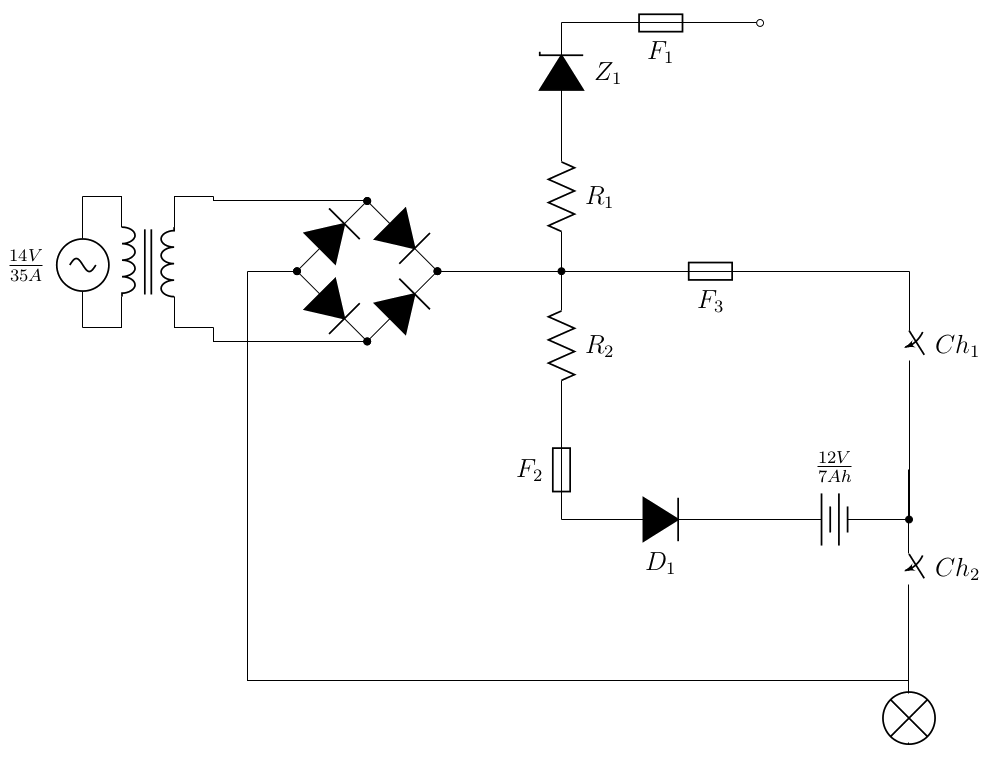
\includegraphics[width=0.8\textwidth]{figuras/alternadorCircuito}
  \caption{Circuito do Alternador}
  \label{fig:figuras_alternadorcircuito}
\end{figure}


% % subsection tac_metro (end)
% \begin{figure}[h]
% 	\centering
% 	\begin{circuitikz}[american,scale=0.8,
% 		start chain=going right,
% 		diamond/.style={
% 			on chain,join,draw,
% 			minimum height=3cm,
% 			text centered,
% 			minimum width=2cm,
% 		},
% 		every join/.style={ultra thick}]

% 	\draw
% 	(-26,0) node[transformer core] (T) {}
% 	(T.A1) node[anchor=east] {} %A1
% 	(T.A2) node[anchor=east] {} %A2
% 	(T.B1) node[anchor=west] {} %B1
% 	(T.B2) node[anchor=west] {} %B2
% 	;

% 	\draw (-23,-1.5)
% 		to[short,n=d1]++(0,0) to [D*,*-*] ++(45 :2)
% 		to[short,n=d2]++(0,0) to [D*,*-*] ++(-45 :2);
% 	\draw (-23,-1.5)
% 		to[short,n=d3]++(0,0) to [D*,*-*] ++(-45 :2)
% 		to[short,n=d4]++(0,0) to [D*,*-*] ++(45:2) to[short,n=_d4]++(0:0)
% 		;

% 	\draw
% 	(T.A2) to  [sinusoidal current source,l^=$\frac{14V}{35A}$,n=cap] ++(0,2.5) to  (T.A1)
% 	(T.B1) |- (d2)
% 	(T.B2) |- (d4)
% 	(_d4) to [short,n=center] ++(5,0)
% 	(center) to [R,l_=$R_1$,*-] ++(0,3) to [zD*,l_=$Z_1$]++(0,2) to [fuse,l_=$F_1$,-o]++(4,0)
% 	(center) to [R,l_=$R_2$,mirror]++(0,-3) to [fuse,l_=$F_2$]++(0,-2) to [D*,l_=$D_1$,n=dio]++(4,0) 
% 	(center) to [fuse,l_=$F_3$]++(6,0) to [short]++(1,0) to [cspst,l^=$Ch_1$]++(0,-3) to [short,n=end]++(0,-2) to [battery,l_=$\frac{12V}{7Ah}$,*-]++(-3,0) to (dio)
% 	(end) to [cspst,l^=$Ch_2$]++(0,-4) to [short,n=baixo]++(0,-0.5) to [lamp]++(0,-1)
% 	(d3) to[short]++(-1,0) |- (baixo)
% 	;

% 	\end{circuitikz}
% 	\caption{Circuito do Alternador}
% 	\label{circ}
% \end{figure}